\chapter{Tilanhallinnan menetelmät} \label{Tilanhallinnan menetelmät}
Sekä Reactin kehitystiimi että Reactin ympärille muodostunut kehittäjäyhteisö ovat keksineet ja toteuttaneet erilaisia tilanhallinnan menetelmiä tyypillisten ongelmien ratkaisemiseksi. Menetelmiä ja lähestymistapoja on monenlaisia. Reactiin sisältyy jo entuudestaan menetelmiä tilanhallinnan helpottamiseksi. Toisaalta monimutkaisille ja suurille sovelluksille on tarjolla usean vuoden kehitystä läpikäyneitä täysimittaisia ulkoisia kirjastoja.

Edellisessä luvussa käsiteltiin kahta tilanhallinnassa tyypillisesti esiintyvää ongelmaa. Tässä luvussa käsitellään erilaisia laajalti käytettyjä ja toimiviksi todettuja tilanhallinnan menetelmiä ja niiden käyttötapauksia. Lisäksi niitä sovelletaan edellisessä luvussa käsiteltyihin ongelmiin.

%%
%% Tilan nostaminen
%%

\section{Tilan nostaminen}
\label{Tilan nostaminen}

Eräs tilanhallinnan menetelmä on tilan nostaminen ylöspäin (engl. lifting state up) komponenttipuussa. Tilan nostamisella pyritään siirtämään tila komponentista toiseen, niin että tilan sijainti nousee komponenttipuun hierarkiassa korkeammalle. Toisin sanoen tila siirretään lähimpään vanhempainkomponenttiin \cite{reactdocsliftingstate}. Tällöin se voidaan jakaa luontevasti lapsikomponenteille propseina. Tilan nostamista havainnollistava esitys on nähtävissä kuvassa \ref{fig:lifting}.
\begin{figure}[h]
\centering 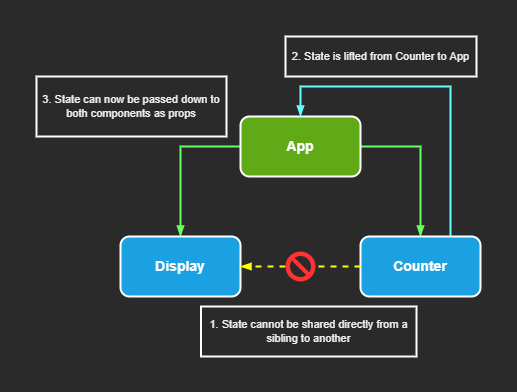
\includegraphics[width=1\textwidth]{kuvat/Lifting state up.png}
\caption{Tilan nostamista havainnollistava kuva.}
\label{fig:lifting} 
\end{figure}

Tilan nostaminen on yksinkertainen ja useimmiten helposti toteutettavissa oleva ratkaisu luvussa \ref{Jakaminen samalla tasolla} esitettyyn ongelmaan, jossa komponenttipuun samalla tasolla sijaitseva komponentti tarvitsee viereisen komponentin hallinnoimaa tilaa. Se on erityisen toimiva ja nopea ratkaisu pienemmissä sovelluksissa, sillä kyseisen menetelmän käyttöönotto ei vaadi minkäänlaisia ulkoisia kirjastoja. Tarkemmin ajateltuna tilan nostaminen on ajattelumalli, jolla sovellus voidaan mukauttaa uuden toiminnallisuuden lisäämiseen tai korjata sovelluksen suunnittelussa tapahtunut suunnitteluvirhe.

%%
%% Kokoonpano ja periminen
%%

\section{Kokoonpano ja periminen}
\label{Kokoonpano ja periminen}

Luvussa \ref{Kaukana oleva käyttökohde} käsiteltiin ongelmaa, jossa tilaa tarvitseva käyttökohde on tilaa hallinnoivasta komponentista usean komponenttikerroksen verran etäällä. Tähän on saatavilla Reactiin jo valmiiksi sisältyvä ratkaisu. Komponenttien kokoonpanolla voidaan välttyä propsien välittämisestä usean komponenttikerroksen läpi, jolloin tila voidaan antaa suoraan sitä tarvitsevalle komponentille. \cite{reactdocscomposition}
\inputminted[bgcolor=black,highlightlines={6,12},highlightcolor=darkgray]{jsx.py:JsxLexer -x}{listaukset/composition1.js}
Esimerkissä esiintyvä komponentti \texttt{Dashboard} ei vastaanota propseja edeltävien komponenttiesimerkkien tavoin. Sen sijaan se vastaanottaa erityisen ennalta nimetyn propsin \texttt{children}. \texttt{Children} mahdollistaa React-elementtien sijoittamisen suoraan komponentin ulostuloon. On myös mainitsemisen arvoista, että komponenttien kokoonpanon käyttö ei poissulje muiden propsien käyttöä \cite{reactdocscomposition}. Esimerkissä käytetty \texttt{Dashboard}-komponentti kirjoitetaan seuraavalla tavalla:
\inputminted[bgcolor=black,highlightlines={4},highlightcolor=darkgray]{jsx.py:JsxLexer -x}{listaukset/composition2.js}
Kokoonpanon hyödyntäminen React-sovelluksessa on erinomainen tapa välttyä tilan jakamiselta usean komponenttikerroksen läpi. Tämän lisäksi kokoonpano voi mahdollistaa suuremmissa ja monimutkaisemmissa sovelluksissa kehittäjälle eräänlaisen lintuperspektiivin, jolla kehittäjä voi tarkastella sovellusta ja sen osia korkealta komponenttipuun näkökulmasta.

%%
%% Flux-arkkitehtuuri
%%

\section{Flux-arkkitehtuuri}
\label{Flux-arkkitehtuuri}

Flux-arkkitehtuuri on Metan kehittämä suunnittelumalli, joka suunniteltiin mahdollistamaan yksisuuntainen tiedon välitys \cite[174]{learningreact}. Flux eroaa oleellisesti yleisesti käytetystä MVC-arkkitehtuurista (sanoista model-view-controller), mutta sisältää samankaltaisia periaatteita, kuten kontrollerin ja näkymän. MVC-arkkitehtuuria hyödyntävässä sovelluksessa kontrolleri toimii välikätenä mallille ja näkymälle. Tämän sijasta Flux-arkkitehtuuria hyödyntävä sovellus käyttää yksisuuntaista datan kulkua, jossa React-komponentit toimivat ikään kuin kontrolleri-näkymä -yhdistelminä \cite{facebookflux} \cite[174]{learningreact} \cite{flux2}. Flux ei ole JavaScript-kehys tai -kirjasto kuten React \cite[5]{flux}. Sitä voisi kuvailla eräänlaisena tiedonhallinnan mallina tai ajattelutapana, joka jakaa tiedon muutokset konkreettisiin toimenpiteisiin sekä mahdollistaa laajojen ja monimutkaisten sovelluksien yksinkertaisemman skaalautumisen \cite[6]{flux}.

Flux-arkkitehtuuri koostuu käytännössä neljästä osasta, joiden välityksellä data liikkuu ja muuttuu. Kuten kuvasta \ref{fig:flux1} on nähtävissä, datan kulku on yksisuuntaista. Tämä mahdollistaa yksinkertaisen yhdessä paikassa hallinnoidun tiedon päivittämisen, joka kulkee aina ennalta määritetyn prosessin läpi.

\begin{figure}[h]
\centering 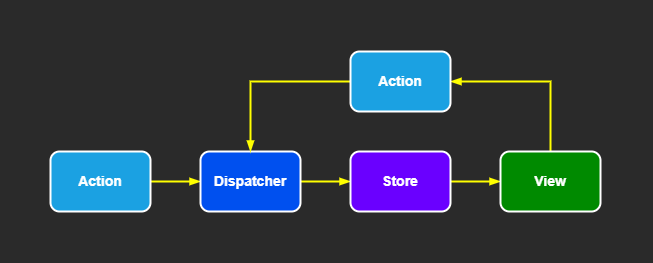
\includegraphics[width=1\textwidth]{kuvat/Flux3.png}
\caption{Flux-arkkitehtuuri yksinkertaistettuna. \cite{facebookflux}}
\label{fig:flux1} 
\end{figure}

%%
%% Action
%%

\subsubsection{Action}
\label{Action}

Actionit, eli toimenpiteet ovat olioita, joihin sisällytetään tilan päivittämiseen tarvittavaa uutta dataa sekä actionin tunnistukseen käytettävä ominaisuus (engl. type property). Kyseisen ominaisuuden määrittäminen on välttämätöntä, sillä se mahdollistaa actionin tunnistamisen. Tunnistamisen kautta voidaan määritellä tietyn tyyppisille actioineille omat vaikutuksensa tilan muutokseen \cite{facebookflux}. Esimerkiksi aiemmin tutkielmassa käytetty laskuriesimerkki voisi napin painalluksella tuottaa actionin, joka sisältää arvon yksi. Tämä ei yksinään riitä määrittämään, että mitä arvolla tulisi tehdä. Tästä syystä actioniin sisällytettäisiin ominaisuus, jolla se voitaisiin tunnistaa joko vähennys- tai summaustoimenpiteeksi. Yksinkertaistettuna action on mekanismi, jolla uutta tietoa lähetetään järjestelmään \cite[12]{flux}.

%%
%% Dispatcher
%%

\subsubsection{Dispatcher}
\label{Dispatcher}

Dispatcher, eli lähettäjä on Flux-arkkitehtuurissa vastuussa actionien eteenpäin lähettämisestä. Niiden tehtävänä on määrittää päivitettävän tiedon sijainti sekä varmistaa, että päivitys tapahtuu oikein. Dispatcherin vastuulla on myös varmistaa, että tila päivittyy vasta kun sille asetetut riippuvuudet täyttyvät. \cite[13]{flux}

%%
%% Store
%%

\subsubsection{Store}
\label{Store}

Flux-arkkitehtuuria käyttävässä sovelluksella tila sijaitsee säiliössä (engl. store). Aiemmin tila on kuvattu aina sidottuna johonkin komponenttiin. Flux-arkkitehtuurissa tila sijaitsee komponenttien ulkopuolella erillisessä keskitetyssä säiliössä. Säiliö voi tavallisen tilan mukaisesti sisältää useita eri arvoja. Flux-arkkitehtuurissa tilan päivittämiseen vaadittu logiikka sijaitsee säiliössä. \cite[14]{flux}

%%
%% View
%%

\subsubsection{View}
\label{View}

View, eli näkymä on Flux-arkkitehtuurissa tiedon esittävä komponentti. Mikäli komponentille on jaettu pääsy tilaa hallinoivaan storeen, voi komponentti näyttää käyttäjälle sen hallinnoivia tietoja. Storea voidaan päivittää kyseisestä komponentista, jolloin käytännössä luodaan uusi action, joka lähetetään dispatcherille. \cite[15]{flux}

%%
%% useReducer
%%

\section{useReducer}
\label{useReducer}

Tutkielman luvussa \ref{Monimutkainen tila} käsiteltiin ongelmaa, jossa sovelluksen tulee hallinnoida monimutkaista tilaa, jossa on erilaisia muuttujia ja tietotyyppejä. Tilan monimutkaistuessa komponenttiin kirjoitetusta koodista yhä suurempi osa on tilan päivittämiseen tarkoitettua logiikkaa. Kuten aiemmin todettiin, tämä ei ole sovelluksen skaalautuvuuden kannalta käytännöllistä. Kyseisen ongelman ehkäisemiseksi Reactiin on sisällytetty mahdollisuus reducerien käyttöön.

Reducerit ovat funktioita, jotka vastaanottavat parametreina nykyisen tilan sekä luvussa \ref{Action} kuvatun actionin ja palauttavat lopuksi uuden päivitetyn tilan. Reduceriin voidaan kirjoittaa kaikki tilan päivittämiseen vaadittu logiikka, jolloin sitä ei tarvitse sisällyttää komponenttiin ollenkaan. Tällöin monimutkaisen tilan päivittäminen tehdään komponentin näkökulmasta toisaalla. Reducerit voidaan kirjoittaa komponenteista täysin riippumattomina konkreettisina funktioina, eikä kehittäjän tarvitse miettiä tilan päivittämisen logiikkaa komponenttia kirjoittaessa. Riittää, että kehittäjällä on tiedossa erilaisille actioneille määritetyt tyypit, jotta tilaa voidaan päivittää oikealla tavalla. \cite{reducer}

Reactin version 16.8 mukana tulleiden hookien joukossa Reactin stabiiliin versioon lisättiin \texttt{useReducer}-hook \cite{reactdocshooksapi}. \texttt{useReducer} mahdollistaa reducerien käytön hookin muodossa. Kyseisen hookin käyttöönotto tehdään kutsumalla \texttt{useReducer}-funktioita, joka vastaanottaa parametreinaan reducer-funktion nimen sekä alkutilan. \texttt{useReducer} palauttaa \texttt{useState}-funktion tavoin kaksi alkioita sisältävän taulukon:
\inputminted[bgcolor=black,highlightlines={13},highlightcolor=darkgray]{jsx.py:JsxLexer -x}{listaukset/usereducer.js}
Esimerkissä ensimmäinen arvo \texttt{state} sisältää tilan. Toinen arvo \texttt{dispatch} on funktio, jota kutsumalla tilaa voidaan päivittää. \texttt{Dispatch} vastaanottaa parametrinaan actionin.

%%
%% useContext
%%

\section{useContext}
\label{useContext}

Tyypillisesti React sovelluksessa tietoa välitetään yksisuuntaisesti alaspäin komponenttipuussa. Kuten tutkielman aiemmissa osissa on todettu, komponentit keskustelevat ja jakavat tietoa keskenään propsien avulla. Useimmiten tämä on täysin toimiva ratkaisu, mutta useassa eri komponentissa vaadittu tieto voi kuitenkin käydä tilanhallinnan kannalta ongelmalliseksi. Esimerkki tällaisesta tiedosta voisi olla sivuston käyttöliittymän teeman määrittävä tila, joka vaikuttaa lähestulkoon jokaiseen käyttöliittymän komponenttiin. \cite{reactdocscontext}

Konteksti (engl. context) on Reactiin sisällytetty rajapinta ja tilanhallinnan menetelmä, jolla tietoa voidaan välittää komponenteille jakamatta sitä jokaisen komponenttipuun kerroksen läpi \cite{reactdocscontext}. Käytännössä konteksti on säiliö sovelluksen eri tilamuttujille, joka voidaan jakaa komponenttipuussa halutuille kerroksille. Mikäli konteksti kattaa koko sovelluksen, on kyseessä globaali konteksti (engl. global context), johon sisällytettyä tilaa kutsutaan globaaliksi tilaksi (engl. global state). Kontekstin käyttö soveltuu joissain tilanteissa ratkaisuksi luvussa \ref{Kaukana oleva käyttökohde} käsiteltyyn ongelmaan, jossa tilaa tarvitseva komponentti on tilaa hallinnoivan komponentin näkökulmasta hyvin kaukana ja syvällä komponenttipuussa. Kontekstin pääasiallinen käyttötapaus on tilanteessa, jossa tilaa tarvitaan useassa eri komponentissa, mutta sen jakaminen jokaiselle sitä tarvitsevalle komponentille ei ole tehokkuuden kannalta käytännöllistä \cite{reactdocscontext}.

On kuitenkin mainitsemisen arvoista, että kontekstia ei kannata käyttää kaikissa tilanteissa. Kontekstin käyttö voi vaikeuttaa komponenttien uudelleenkäyttömahdollisuuksia \cite{reactdocscontext}. Mikäli komponentti on riippuvainen kontekstista, on sillä aina oltava pääsy kontekstiin. Tällaisessa tilanteessa kontekstista riippuvainen komponentti ei toimi, eikä sitä voi käyttää kontekstin ulkopuolella. Kontekstia tulisi käyttää vain tilanteissa, joissa tilaa tarvitseva komponentti on todella syvällä komponenttipuussa \cite{kentcdodds2}. Luvussa \ref{Kokoonpano ja periminen} käsitelty kokoonpano ja periminen on useimmiten parempi ratkaisu tilanteeseen, jossa halutaan välttyä tilan jakamiselta usean komponenttikerroksen läpi \cite{reactdocscontext}.

Edellä mainittu sovelluksen teeman määrittävä tila on erinomainen kontekstin käyttötapaus \cite[112]{buglreacthooks}. Teeman vaihtuessa tyypillisesti kaikki sovelluksen komponentit muuttuvat tyyliltään tai väritykseltään. Tällöin voi olla järkevää sisällyttää teemaa hallinnoiva tila kontekstiin. Kontekstin käyttöönotto tehdään tällaisessa tapauksessa luomalla kontekstiolio seuraavan esimerkin tavoin:
\inputminted[bgcolor=black,highlightlines={5,9-11,20},highlightcolor=darkgray,samepage]{jsx.py:JsxLexer -x}{listaukset/usecontext.js}
Esimerkissä kontekstiolio luodaan rivillä 5 kutsumalla \texttt{createContext}-funktiota, jolle annetaan parametrina alkutila. Tämän jälkeen määritellään alue, jonka konteksti kattaa. Alueen sisällä olevat komponentit saavat käyttöoikeuden kontekstin sisältöön. Tämä on tehty esimerkissä riveillä 9-11, joissa aiemmin luotuun kontekstiolioon sisältyvää React-elementtiä \texttt{Provider} käytetään tähän tarkoitukseen. \texttt{Provider}-elementille annetaan propsina \texttt{value}, johon asetetaan kontekstin sisällä jaettava tila. Nyt kontekstin \texttt{Provider}-elementin sisällä olevat komponentit voivat käyttää kontekstin \texttt{value} propsin arvoa \texttt{useContext}-hookilla, kuten esimerkissä on tehty rivillä 20. Tällöin \texttt{value} propsin muuttuessa sitä käyttävät komponentit uudelleenrenderöidään. 

%%
%% Redux-kirjasto
%%

\section{Redux-kirjasto}
\label{Redux-kirjasto}

Redux on vuonna 2015 julkaistu tilan säilöntään ja hallintaan suunnattu kirjasto, joka mahdollistaa ennakoitavan tilan mutatoitumisen uhraamatta asynkronisuuden tuomia suorituskykyetuja \cite[8]{learningredux}. Sen alkuperäiset kehittäjät ovat Andrew Clark ja Dan Abramov, jotka työskentelevät tutkielman kirjoitushetkellä osana Reactin virallista kehitystiimiä \cite{reactdocsteam} \cite[183]{learningreact}.

Redux perustuu pitkälti luvussa \ref{Flux-arkkitehtuuri} käsiteltyyn Metan luomaan Flux-arkkitehtuuriin. Tästä syystä Reduxia pidetäänkin yhtenä suosituimpana Flux-arkkitehtuurin implementaationa \cite[183]{learningreact}. Flux-arkkitehtuurista poiketen Redux hyödyntää usean storen sijasta yhtä storea, joka sisältää koko sovelluksen toiminnallisuuden edellyttämän tilan \cite[13]{learningredux}. Reduxille dispatcher on käsitteenä vieras. Sen sijaan Redux käyttää tilan päivittämiseen luvussa \ref{useReducer} käsitellyn useReducer-hookin tapaista reducer-funktiota. Tyypillisesti sovelluksen kasvaessa reducereita aletaan jakaa pienempiin yksittäisiin reducereihin, joista jokainen on vastuussa tietystä sovelluksen tilasta. \cite[15]{learningredux} \cite{reduxdocsstore}

Toiminnallisuudeltaan edellisissä luvuissa käsitellyt useReducer- ja useContext-hookit sekä niiden yhdistelmät ovat hyvin samankaltaisia ratkaisuja Reduxiin nähden. Redux on kuitenkin pitkälti tarkemman hienosäädön ja sovelluksen kehityksen mahdollistava ratkaisu. Redux nimittäin mahdollistaa esimerkiksi todella tarkan vianmääritysprosessin, jossa kehittäjä voi seurata tilan muuttumista jokaisella muutoshetkellä ja määrittää tarkalleen vian lähteen sekä syyn. Myös väliohjelmiston (engl. middleware) käyttöönotto on mahdollista Reduxin avulla. Väliohjelmiston avulla kehittäjä kiinnittyä actionin lähetyksen ja reduceriin saapumisen väliin ja lisätä haluamansa toiminnallisuudeen, esimerkiksi sovelluksen kaatumisraportin. \cite{reduxdocsmiddleware}

Reduxin käyttöönotto vaatii kuitenkin luvussa \ref{useContext} käsiteltyyn konteksti-rajapintaan verrattuna enemmän työtä erityisesti sovelluksen alkuvaiheessa. Riippuen sovelluksen arvioidusta monimutkaisuudesta voi Reduxin käyttöönottoon vaadittu työ olla kuitenkin pitkällä aikavälillä kannattavampaa. Keskitetty Reduxilla toteutettu tietosäiliö sekä sitä muokkaavat reducer-funktiot yksinkertaistavat sovelluksen jatkokehitystä, joka on erityisen hyödyllistä erityisesti suuremmissa sovellushankkeissa. \cite[531]{proreact}